\begin{boxD}
    برای این منظور می‌توانیم از معیارهایی چون میانگین پیکسل‌ها ، واریانس پیکسل‌ها و حتی مد پیکسل‌ها نیز استفاده‌کنیم.
\end{boxD}

\begin{boxA}
    ذکر این نکته را قبل از بررسی معیارهای فوق بر روی تصاویر الزامی می‌دانم که به نظر شخصی بنده بعضی تصاویر برچسب مناسبی ندارند.
    حداقل ایهام بالایی در تشخیص تصاویر موجود است.
\end{boxA}

\begin{boxD}
    برای این مساله اولا ذکر این نکته در محاسبات ضرورت دارد که هر کجا برچسب داده با برچسب پیش‌بینی شده مطابقت داشت را به عنوان مقداری برای
    \lr{True Positive}
    درنظرگرفته‌ایم.

    مقادیر
    \lr{False Positive}
    و
    \lr{True Negative}
    نیز بر حسب اتفاق یکی از حالات اشتباه درنظرگرفته‌ایم.

    در هر کدام از ۳ طبقه‌بند زیر یک مقداری را بر حسب مشاهداتی که از این ۸۰ فایل داشتیم ، انتخاب کرده و سپس آن را به عنوان 
    \lr{threshold}
    درنظرمی‌گیریم.
\end{boxD}

\begin{figure}[h]
    \centering
    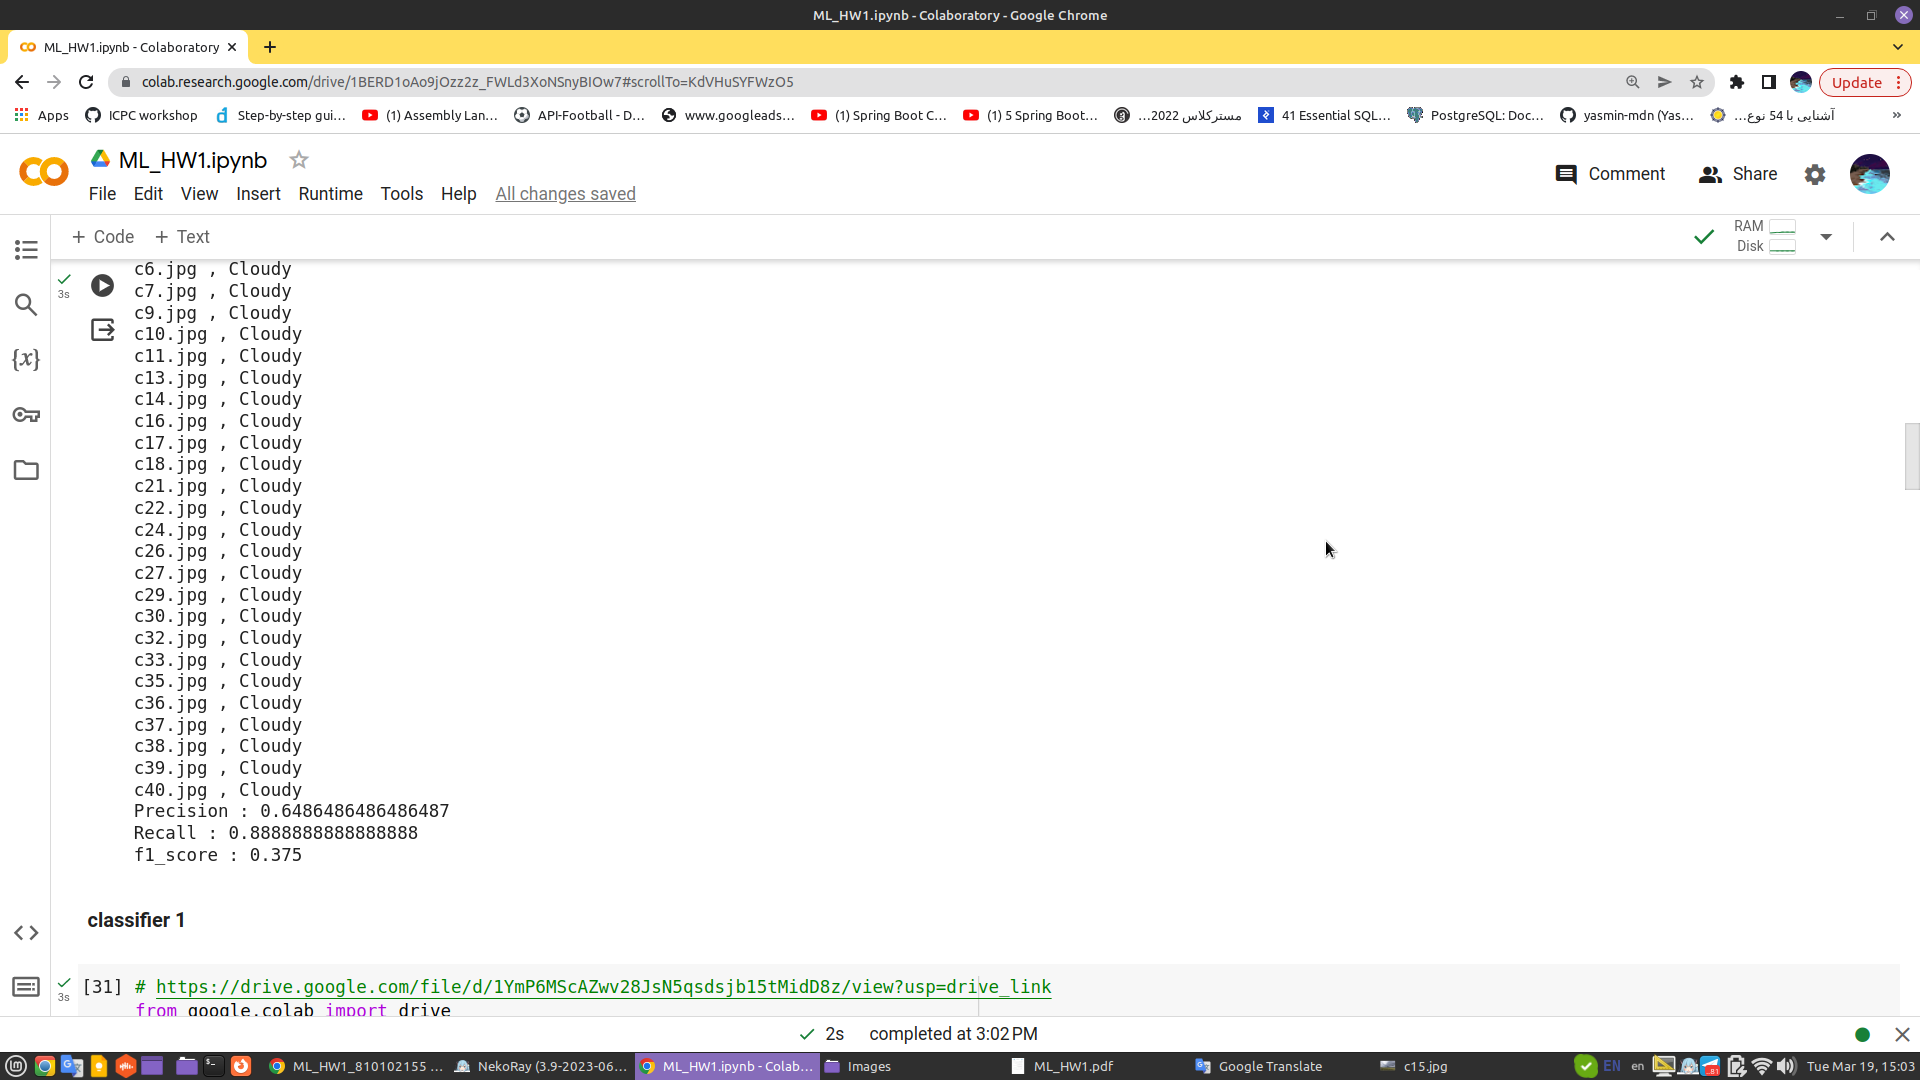
\includegraphics
    [width = 0.8\textwidth]
    {ML1/images/8-classifier0.png}
    \caption{نتایج طبقه‌بندی بر اساس میانگین پیکسل‌ها}
    \label{fig:enter-label}
\end{figure}

\begin{figure}[h]
    \centering
    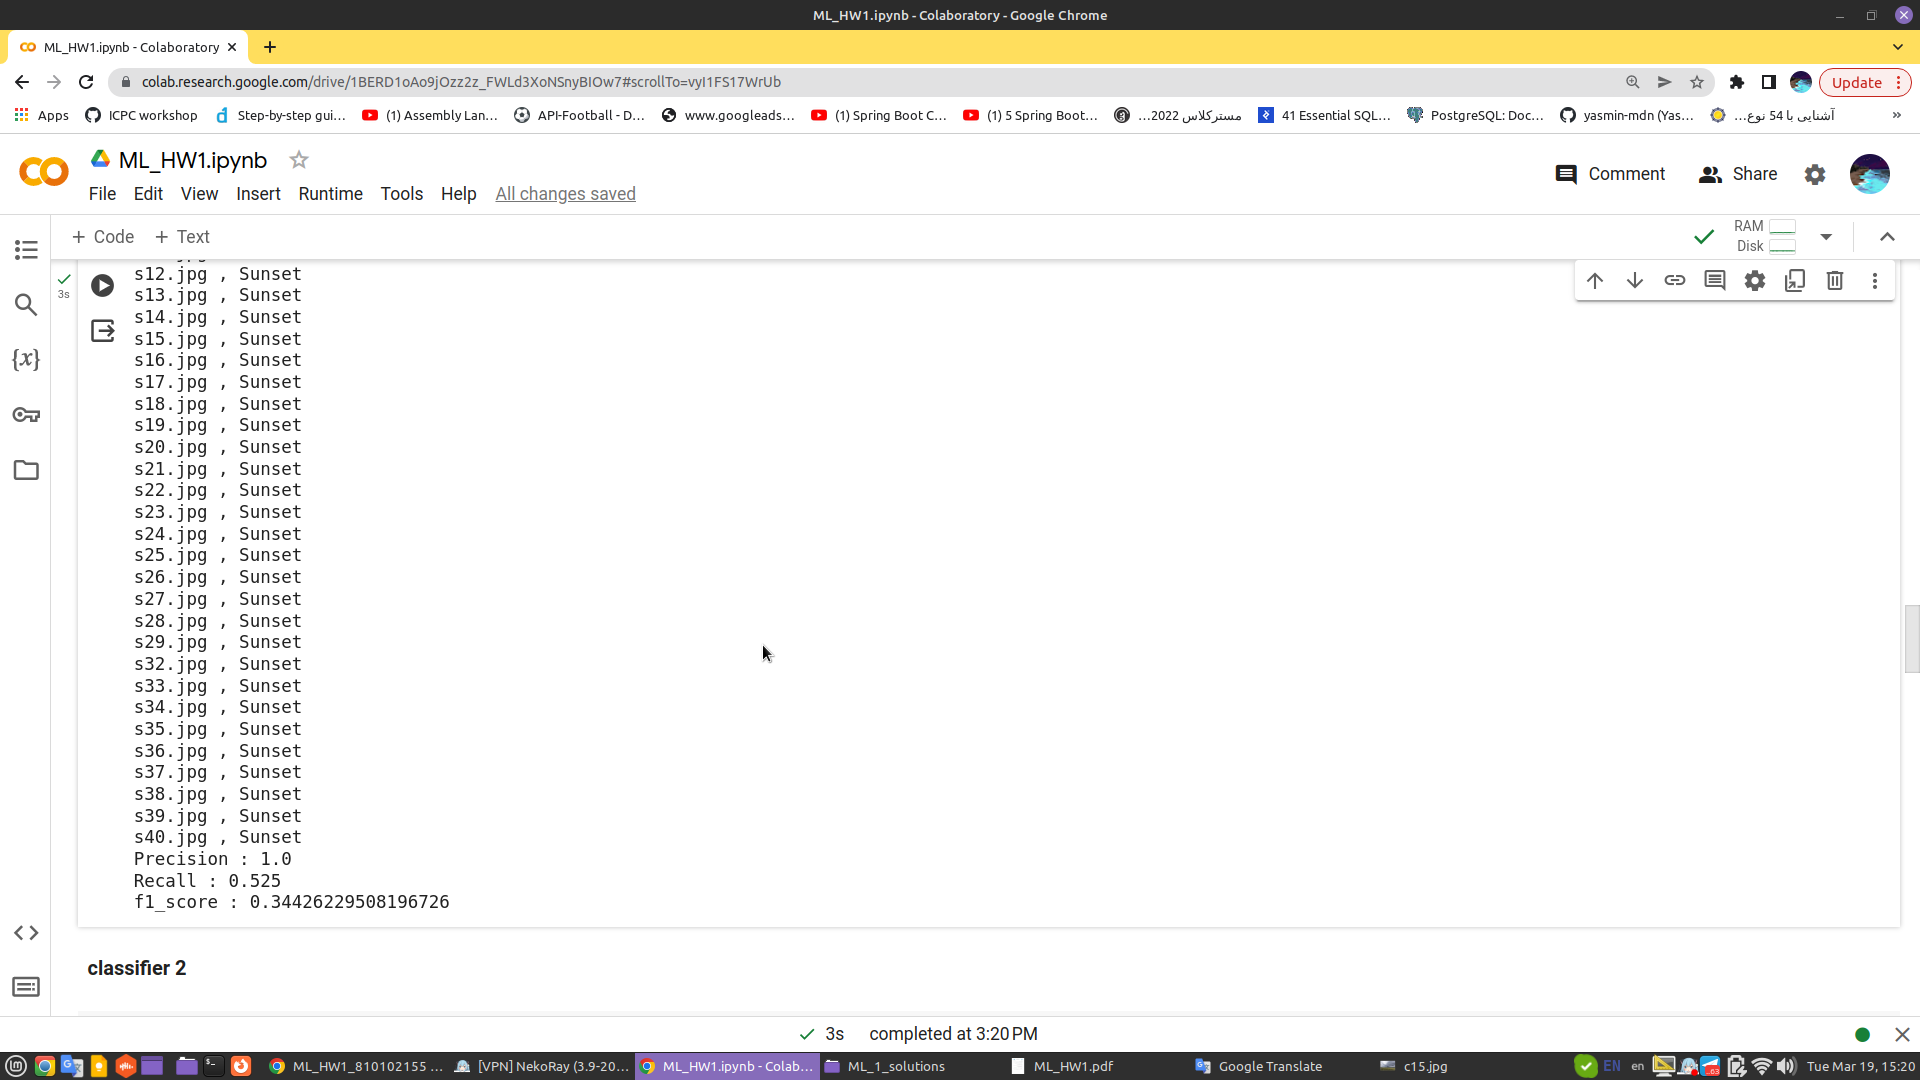
\includegraphics
    [width = 0.8\textwidth]
    {ML1/images/8-classifier1.png}
    \caption{نتایج طبقه‌بندی بر اساس واریانس پیکسل‌ها}
    \label{fig:enter-label}
\end{figure}

\begin{boxD}
    به عنوان مثال طبقه‌بند بر اساس پیکسل‌ها توانسته‌است یک کلاس را به صورت کامل درست تشخیص‌دهد اما در تشخیص کلاس غروب به سختی چند مورد را تشخیص‌داده‌است.
\end{boxD}

\begin{figure}[h]
    \centering
    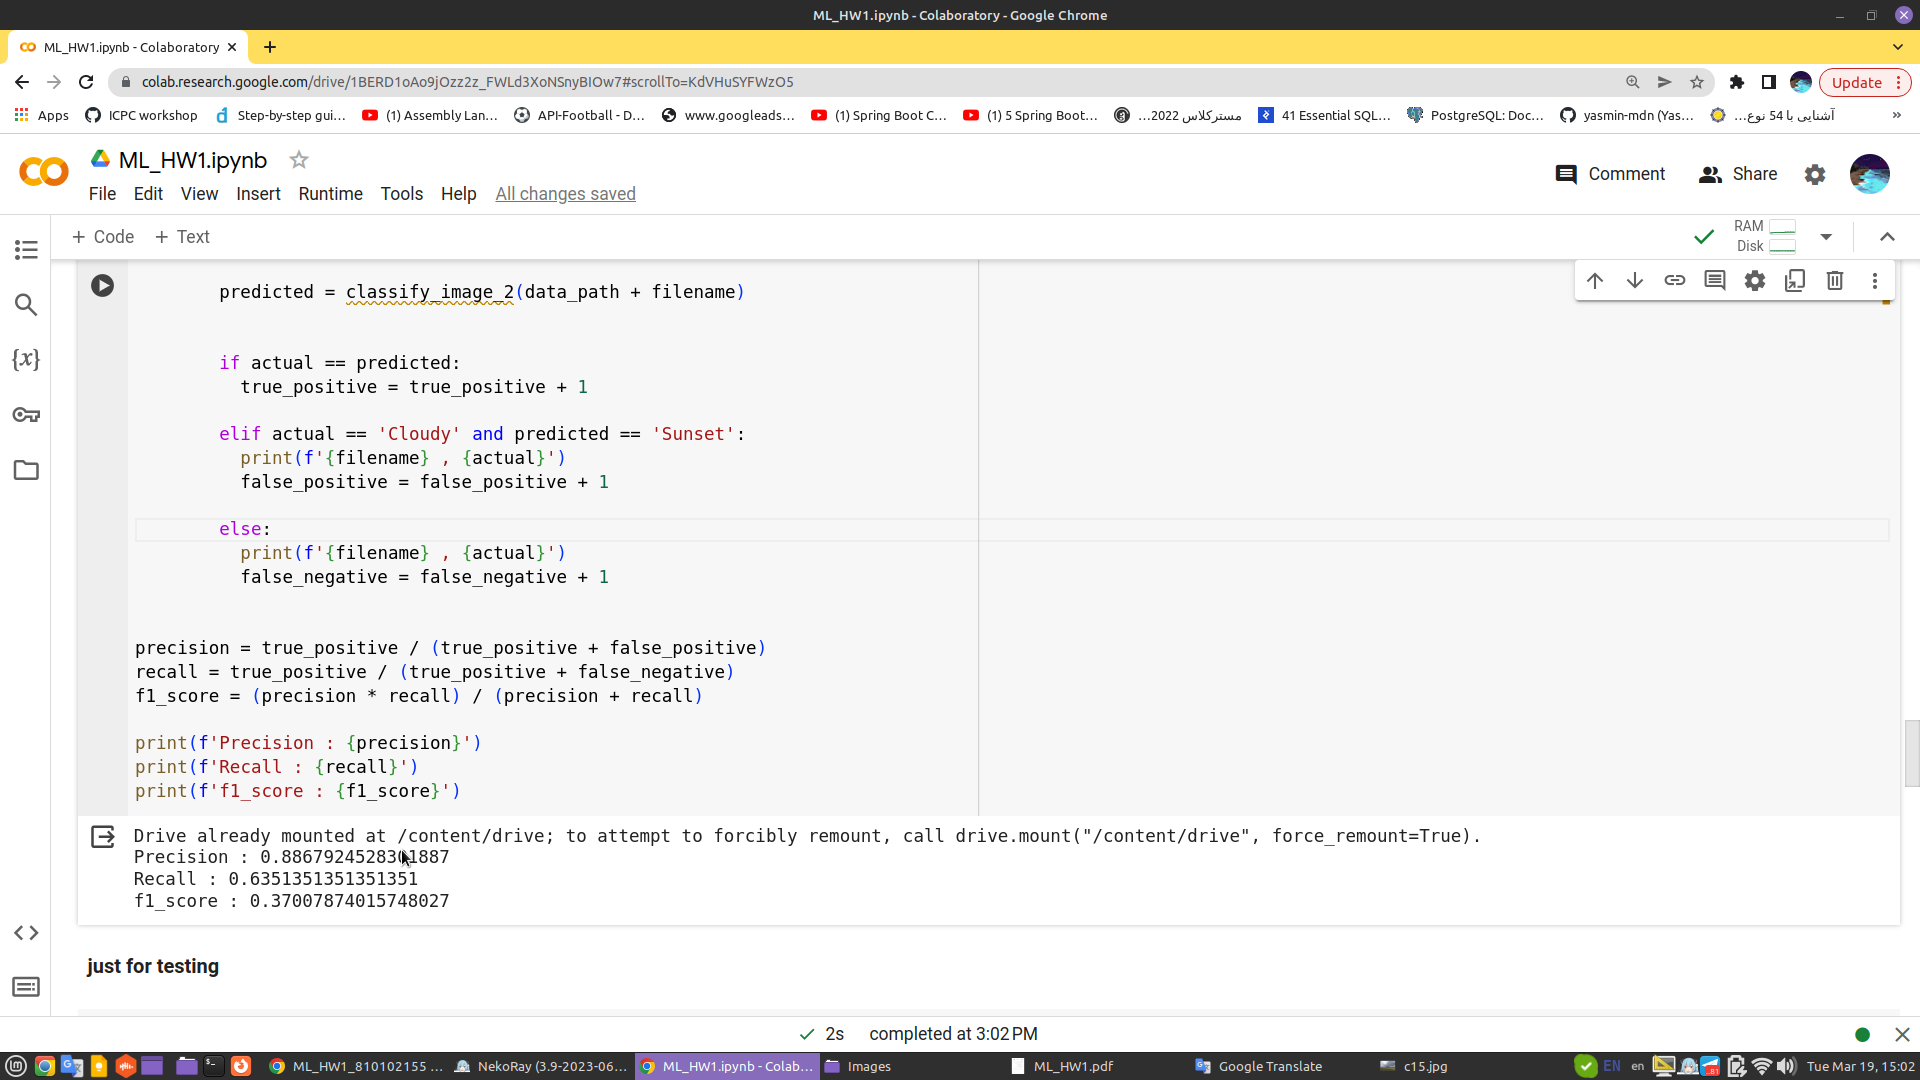
\includegraphics
    [width = 0.8\textwidth]
    {ML1/images/8-classifier2.png}
    \caption{نتایج طبقه‌بندی بر اساس مد پیکسل‌ها}
    \label{fig:enter-label}
\end{figure}

\begin{boxD}
    از محاسبات دقت و بازسپاری اینطور به نظر می‌رسد که معیار مد پیکسل‌ها تا حد خوبی توانسته‌است که جداسازی میان تصاویر را انجام دهد.

    (تصور شخصی من اینطور بود که میانگین پیکسل‌های تصاویر ابری باید به شدت متفاوت از تصاویر غروب باشد ، اما به نسبت عالی عمل نکرد این معیار)

    همچنین اینطور به نظرمی‌رسد که پیکسل با فراوانی بیشتر که همان مد خوانده می‌شود توانسته حدفاصل خوبی برای ایجاد اختلاف بین این دو کلاس از تصاویر ایجاد کند.
\end{boxD}

\begin{boxA}
    به عنوان مثالی دیگر معیار میانگین برای عکس 
    \lr{s8}
    به اشتباه عمل‌کرده‌است . 
    و این امر طبیعی به نظر می‌رسد ، چرا که میزان ابرهای درون تصویر باعث شده است که میانگین پیکسل‌ها در حدود میانگین تصاویر ابری باشد.
\end{boxA}

\begin{boxA}
    معیار واریانس برای هیچ‌کدام از تصاویر غروب به خوبی عمل نکرده‌است . میزان پراکندگی در این داده‌ها به طرز چشمگیری مشهود است.
    همچنین یک بخشی از این اتفاق به‌نظرمن به خاطر برچسب اشتباه بعضی از داده‌ها می‌باشد.
\end{boxA}


\begin{boxA}
    در مورد شاخص مد نیز به عنوان مثال ، تصویر
     \lr{s30}
     که در این تصویر بیشترین فراوانی مربوط به رنگ سفید و ابرها می‌باشد.
     به همین ترتیب تصاویر
     \lr{s9 , s8}.
\end{boxA}